% Generated by pysimcount.figleader -- do not edit; regenerate instead.
% figure: main-total-all-formulas -- source curves (no error bars) with cost at n = 500 beside them
% seeds [1, 2, 3, 4, 5, 6, 7, 8, 9, 10]; metric=total kind=xyz merged (Clifford+Rz (cz), simcount template)
% shown: suzuki4, suzuki6, mo-q6, mo-q14, bm-q10, mo-o8-q21, morales-y8m10, morales-m8
% removed (see main-total-all-formulas-ranking.md): lie-trotter, suzuki2, suzuki8
% n = 500; x = the source record's plotted value; bars min..max over seeds
% cheapest on = seeds on which the formula is cheapest; rank range = min..max of its rank over seeds
% per-seed values: runs' totals if measured, else each seed's own fit c(n) ceil(a_s n^b_s)
% row order (plotted value) ['bm-q10', 'morales-m8', 'mo-q14', 'morales-y8m10', 'mo-q6', 'mo-o8-q21', 'suzuki6', 'suzuki4'] differs from mean-rank order ['morales-m8', 'bm-q10', 'mo-q14', 'morales-y8m10', 'mo-q6', 'mo-o8-q21', 'suzuki6', 'suzuki4']
% left axis: coordinates copied unchanged from the source .tex
% derived: main-total-all-formulas.tex by pysimcount.figleader; source_sha256=2b5f44160ee6506c88d0b5334462cb6e56f47f5b3070c640776edb4f45de8d42
% figure made at git_commit=eed0c490bd2a7ed3c821acf76ae930c79d2195f6 git_dirty=False
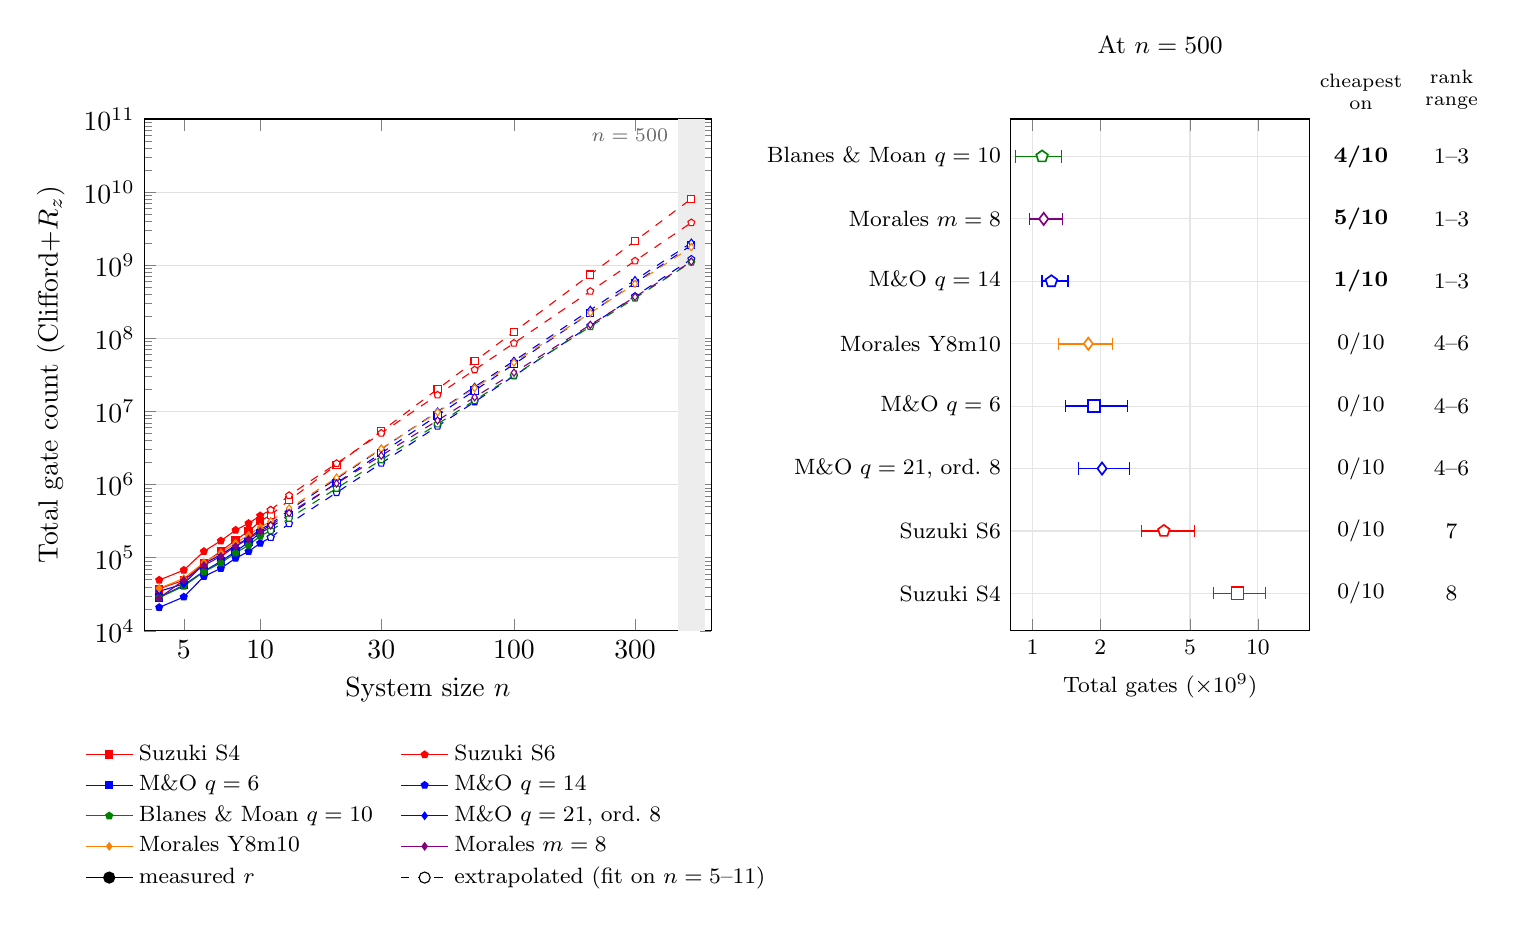
\begin{tikzpicture}
  \begin{loglogaxis}[
    name=main, scale only axis,
    width=7.2cm, height=6.5cm,
    xlabel={System size $n$},
    ylabel={Total gate count (Clifford+$R_z$)},
    xtick={5,10,30,100,300}, xticklabels={5,10,30,100,300},
    xmin=3.5, xmax=600, ymin=10000, ymax=1e+11,
    ymajorgrids=true, grid style={black!12},
    legend style={at={(0.5,-0.2)}, anchor=north, draw=none, font=\footnotesize,
      legend columns=2, /tikz/every even column/.append style={column sep=8pt}},
    legend cell align=left,
  ]
    \fill[black!7] (axis cs:442.478,10000) rectangle (axis cs:565,1e+11);
    \node[anchor=north east, font=\scriptsize, black!60] at (axis cs:442.478,1e+11) {$n=500$};
    % suzuki4: measured n, mean over seeds, bars min..max over seeds
    \addplot[red, solid, mark=square*, mark size=1.3pt, mark options={solid, fill=red}] coordinates {
      (4,37651.2)
      (5,49184)
      (6,84333.6)
      (7,122578)
      (8,174349)
      (9,229914)
      (10,315032)
      (11,384780)
    };
    \addlegendentry{Suzuki S4}
    % suzuki4: extrapolated, r = ceil(3.65267 n^1.59931), per step = 212 n + 0; bars min..max of per-seed fits
    \addplot[red, dashed, mark=square*, mark size=1.3pt, mark options={solid, fill=white}, forget plot] coordinates {
      (11,384780)
      (13,609903)
      (20,1.86772e+06)
      (30,5.3583e+06)
      (50,2.02333e+07)
      (70,4.85565e+07)
      (100,1.22856e+08)
      (200,7.46656e+08)
      (300,2.14644e+09)
      (500,8.12156e+09)
    };
    % suzuki6: measured n, mean over seeds, bars min..max over seeds
    \addplot[red, solid, mark=pentagon*, mark size=1.3pt, mark options={solid, fill=red}] coordinates {
      (4,49536)
      (5,67596)
      (6,121982)
      (7,170486)
      (8,238598)
      (9,295358)
      (10,375648)
      (11,449539)
    };
    \addlegendentry{Suzuki S6}
    % suzuki6: extrapolated, r = ceil(1.63295 n^1.35284), per step = 1032 n + 0; bars min..max of per-seed fits
    \addplot[red, dashed, mark=pentagon*, mark size=1.3pt, mark options={solid, fill=white}, forget plot] coordinates {
      (11,449539)
      (13,711048)
      (20,1.95048e+06)
      (30,5.05577e+06)
      (50,1.68216e+07)
      (70,3.71314e+07)
      (100,8.60482e+07)
      (200,4.40808e+08)
      (300,1.14685e+09)
      (500,3.82702e+09)
    };
    % mo-q6: measured n, mean over seeds, bars min..max over seeds
    \addplot[blue, solid, mark=square*, mark size=1.3pt, mark options={solid, fill=blue}] coordinates {
      (4,28639.6)
      (5,42251)
      (6,65122.2)
      (7,89435.5)
      (8,122250)
      (9,162350)
      (10,219098)
      (11,259376)
    };
    \addlegendentry{M\&O $q=6$}
    % mo-q6: extrapolated, r = ceil(3.93927 n^1.32338), per step = 253 n + 0; bars min..max of per-seed fits
    \addplot[blue, dashed, mark=square*, mark size=1.3pt, mark options={solid, fill=white}, forget plot] coordinates {
      (11,259376)
      (13,387115)
      (20,1.05197e+06)
      (30,2.69749e+06)
      (50,8.84108e+06)
      (70,1.93375e+07)
      (100,4.43307e+07)
      (200,2.22463e+08)
      (300,5.71785e+08)
      (500,1.87899e+09)
    };
    % mo-q14: measured n, mean over seeds, bars min..max over seeds
    \addplot[blue, solid, mark=pentagon*, mark size=1.3pt, mark options={solid, fill=blue}] coordinates {
      (4,20916)
      (5,29050)
      (6,55427.4)
      (7,71579.2)
      (8,98537.6)
      (9,121836)
      (10,158032)
      (11,189174)
    };
    \addlegendentry{M\&O $q=14$}
    % mo-q14: extrapolated, r = ceil(1.412 n^1.28559), per step = 581 n + 0; bars min..max of per-seed fits
    \addplot[blue, dashed, mark=pentagon*, mark size=1.3pt, mark options={solid, fill=white}, forget plot] coordinates {
      (11,189174)
      (13,292301)
      (20,778540)
      (30,1.96088e+06)
      (50,6.28642e+06)
      (70,1.35553e+07)
      (100,3.06013e+07)
      (200,1.49271e+08)
      (300,3.77168e+08)
      (500,1.21287e+09)
    };
    % bm-q10: measured n, mean over seeds, bars min..max over seeds
    \addplot[green!50!black, solid, mark=pentagon*, mark size=1.3pt, mark options={solid, fill=green!50!black}] coordinates {
      (4,28522.8)
      (5,40866)
      (6,64301.4)
      (7,84942.9)
      (8,116093)
      (9,148244)
      (10,197658)
      (11,234854)
    };
    \addlegendentry{Blanes \& Moan $q=10$}
    % bm-q10: extrapolated, r = ceil(2.82314 n^1.2111), per step = 417 n + 0; bars min..max of per-seed fits
    \addplot[green!50!black, dashed, mark=pentagon*, mark size=1.3pt, mark options={solid, fill=white}, forget plot] coordinates {
      (11,234854)
      (13,345318)
      (20,890712)
      (30,2.17924e+06)
      (50,6.7408e+06)
      (70,1.41863e+07)
      (100,3.12333e+07)
      (200,1.44899e+08)
      (300,3.55684e+08)
      (500,1.10288e+09)
    };
    % mo-o8-q21: measured n, mean over seeds, bars min..max over seeds
    \addplot[blue, solid, mark=diamond*, mark size=1.3pt, mark options={solid, fill=blue}] coordinates {
      (4,34720)
      (5,43834)
      (6,83328)
      (7,109976)
      (8,147907)
      (9,185144)
      (10,243908)
      (11,289304)
    };
    \addlegendentry{M\&O $q=21$, ord.~8}
    % mo-o8-q21: extrapolated, r = ceil(1.3736 n^1.30758), per step = 868 n + 0; bars min..max of per-seed fits
    \addplot[blue, dashed, mark=diamond*, mark size=1.3pt, mark options={solid, fill=white}, forget plot] coordinates {
      (11,289304)
      (13,447975)
      (20,1.20652e+06)
      (30,3.07012e+06)
      (50,9.96898e+06)
      (70,2.16609e+07)
      (100,4.93545e+07)
      (200,2.44759e+08)
      (300,6.24778e+08)
      (500,2.03494e+09)
    };
    % morales-y8m10: measured n, mean over seeds, bars min..max over seeds
    \addplot[orange, solid, mark=diamond*, mark size=1.3pt, mark options={solid, fill=orange}] coordinates {
      (4,38192)
      (5,52080)
      (6,85932)
      (7,116659)
      (8,158323)
      (9,203893)
      (10,260400)
      (11,315084)
    };
    \addlegendentry{Morales Y8m10}
    % morales-y8m10: extrapolated, r = ceil(1.66328 n^1.25438), per step = 868 n + 0; bars min..max of per-seed fits
    \addplot[orange, dashed, mark=diamond*, mark size=1.3pt, mark options={solid, fill=white}, forget plot] coordinates {
      (11,315084)
      (13,472800)
      (20,1.24645e+06)
      (30,3.10136e+06)
      (50,9.79104e+06)
      (70,2.09257e+07)
      (100,4.67678e+07)
      (200,2.23423e+08)
      (300,5.58089e+08)
      (500,1.76907e+09)
    };
    % morales-m8: measured n, mean over seeds, bars min..max over seeds
    \addplot[violet, solid, mark=diamond*, mark size=1.3pt, mark options={solid, fill=violet}] coordinates {
      (4,28160)
      (5,49280)
      (6,78566.4)
      (7,104474)
      (8,143053)
      (9,180576)
      (10,229504)
      (11,278010)
    };
    \addlegendentry{Morales $m=8$}
    % morales-m8: extrapolated, r = ceil(2.19247 n^1.17079), per step = 704 n + 0; bars min..max of per-seed fits
    \addplot[violet, dashed, mark=diamond*, mark size=1.3pt, mark options={solid, fill=white}, forget plot] coordinates {
      (11,278010)
      (13,409094)
      (20,1.03629e+06)
      (30,2.49427e+06)
      (50,7.54688e+06)
      (70,1.5671e+07)
      (100,3.39891e+07)
      (200,1.53176e+08)
      (300,3.69558e+08)
      (500,1.12147e+09)
    };
    \addlegendimage{black, solid, mark=*, mark options={solid, fill=black}}
    \addlegendentry{measured $r$}
    \addlegendimage{black, dashed, mark=*, mark options={solid, fill=white}}
    \addlegendentry{extrapolated (fit on $n = 5$--$11$)}
  \end{loglogaxis}
  \begin{semilogxaxis}[
    scale only axis, clip=false,
    at={(11.0cm,0cm)}, anchor=south west,
    width=3.8cm, height=6.5cm,
    title={At $n = 500$}, title style={font=\small, yshift=14pt},
    xlabel={Total gates ($\times 10^{9}$)}, xlabel style={font=\footnotesize},
    xmin=8e+08, xmax=1.7e+10, xtick={1e+09,2e+09,5e+09,1e+10}, xticklabels={1,2,5,10},
    xminorticks=false,
    y dir=reverse, ymin=0.4, ymax=8.6, ytick={1,2,3,4,5,6,7,8},
    yticklabels={{Blanes \& Moan $q=10$},{Morales $m=8$},{M\&O $q=14$},{Morales Y8m10},{M\&O $q=6$},{M\&O $q=21$, ord.~8},{Suzuki S6},{Suzuki S4}},
    tick label style={font=\footnotesize}, ytick style={draw=none},
    xmajorgrids=true, ymajorgrids=true, grid style={black!10},
  ]
    % bm-q10: plotted 1.10288e+09, seeds 8.43591e+08..1.34816e+09, cheapest on 4/10, rank 1..3
    \addplot[green!50!black, only marks, mark=pentagon*, mark size=2.2pt, mark options={solid, fill=white, line width=0.6pt}, error bars/.cd, x dir=both, x explicit, error bar style={solid, line width=0.6pt}] coordinates {
      (1.10288e+09,1) += (2.45279e+08,0) -= (2.59291e+08,0)
    };
    % morales-m8: plotted 1.12147e+09, seeds 9.65888e+08..1.36541e+09, cheapest on 5/10, rank 1..3
    \addplot[violet, only marks, mark=diamond*, mark size=2.2pt, mark options={solid, fill=white, line width=0.6pt}, error bars/.cd, x dir=both, x explicit, error bar style={solid, line width=0.6pt}] coordinates {
      (1.12147e+09,2) += (2.43936e+08,0) -= (1.55584e+08,0)
    };
    % mo-q14: plotted 1.21287e+09, seeds 1.10187e+09..1.43739e+09, cheapest on 1/10, rank 1..3
    \addplot[blue, only marks, mark=pentagon*, mark size=2.2pt, mark options={solid, fill=white, line width=0.6pt}, error bars/.cd, x dir=both, x explicit, error bar style={solid, line width=0.6pt}] coordinates {
      (1.21287e+09,3) += (2.24527e+08,0) -= (1.11e+08,0)
    };
    % morales-y8m10: plotted 1.76907e+09, seeds 1.31025e+09..2.27156e+09, cheapest on 0/10, rank 4..6
    \addplot[orange, only marks, mark=diamond*, mark size=2.2pt, mark options={solid, fill=white, line width=0.6pt}, error bars/.cd, x dir=both, x explicit, error bar style={solid, line width=0.6pt}] coordinates {
      (1.76907e+09,4) += (5.02485e+08,0) -= (4.58825e+08,0)
    };
    % mo-q6: plotted 1.87899e+09, seeds 1.39555e+09..2.63917e+09, cheapest on 0/10, rank 4..6
    \addplot[blue, only marks, mark=square*, mark size=2.2pt, mark options={solid, fill=white, line width=0.6pt}, error bars/.cd, x dir=both, x explicit, error bar style={solid, line width=0.6pt}] coordinates {
      (1.87899e+09,5) += (7.60176e+08,0) -= (4.83445e+08,0)
    };
    % mo-o8-q21: plotted 2.03494e+09, seeds 1.59669e+09..2.69123e+09, cheapest on 0/10, rank 4..6
    \addplot[blue, only marks, mark=diamond*, mark size=2.2pt, mark options={solid, fill=white, line width=0.6pt}, error bars/.cd, x dir=both, x explicit, error bar style={solid, line width=0.6pt}] coordinates {
      (2.03494e+09,6) += (6.56295e+08,0) -= (4.38253e+08,0)
    };
    % suzuki6: plotted 3.82702e+09, seeds 3.05936e+09..5.23534e+09, cheapest on 0/10, rank 7..7
    \addplot[red, only marks, mark=pentagon*, mark size=2.2pt, mark options={solid, fill=white, line width=0.6pt}, error bars/.cd, x dir=both, x explicit, error bar style={solid, line width=0.6pt}] coordinates {
      (3.82702e+09,7) += (1.40832e+09,0) -= (7.67653e+08,0)
    };
    % suzuki4: plotted 8.12156e+09, seeds 6.37431e+09..1.07703e+10, cheapest on 0/10, rank 8..8
    \addplot[red, only marks, mark=square*, mark size=2.2pt, mark options={solid, fill=white, line width=0.6pt}, error bars/.cd, x dir=both, x explicit, error bar style={solid, line width=0.6pt}] coordinates {
      (8.12156e+09,8) += (2.64878e+09,0) -= (1.74725e+09,0)
    };
    \node[anchor=south, font=\scriptsize, align=center] at ([xshift=0.65cm]axis cs:1.7e+10,0.4) {cheapest\\on};
    \node[anchor=south, font=\scriptsize, align=center] at ([xshift=1.8cm]axis cs:1.7e+10,0.4) {rank\\range};
    \node[font=\footnotesize\bfseries] at ([xshift=0.65cm]axis cs:1.7e+10,1) {4/10};
    \node[font=\footnotesize] at ([xshift=1.8cm]axis cs:1.7e+10,1) {1--3};
    \node[font=\footnotesize\bfseries] at ([xshift=0.65cm]axis cs:1.7e+10,2) {5/10};
    \node[font=\footnotesize] at ([xshift=1.8cm]axis cs:1.7e+10,2) {1--3};
    \node[font=\footnotesize\bfseries] at ([xshift=0.65cm]axis cs:1.7e+10,3) {1/10};
    \node[font=\footnotesize] at ([xshift=1.8cm]axis cs:1.7e+10,3) {1--3};
    \node[font=\footnotesize] at ([xshift=0.65cm]axis cs:1.7e+10,4) {0/10};
    \node[font=\footnotesize] at ([xshift=1.8cm]axis cs:1.7e+10,4) {4--6};
    \node[font=\footnotesize] at ([xshift=0.65cm]axis cs:1.7e+10,5) {0/10};
    \node[font=\footnotesize] at ([xshift=1.8cm]axis cs:1.7e+10,5) {4--6};
    \node[font=\footnotesize] at ([xshift=0.65cm]axis cs:1.7e+10,6) {0/10};
    \node[font=\footnotesize] at ([xshift=1.8cm]axis cs:1.7e+10,6) {4--6};
    \node[font=\footnotesize] at ([xshift=0.65cm]axis cs:1.7e+10,7) {0/10};
    \node[font=\footnotesize] at ([xshift=1.8cm]axis cs:1.7e+10,7) {7};
    \node[font=\footnotesize] at ([xshift=0.65cm]axis cs:1.7e+10,8) {0/10};
    \node[font=\footnotesize] at ([xshift=1.8cm]axis cs:1.7e+10,8) {8};
  \end{semilogxaxis}
\end{tikzpicture}
